\hypertarget{conceptos-previos}{%
\section{Conceptos previos}\label{conceptos-previos}}

Este documento resume las páginas 135 a 141 de los apuntes.

Recordemos que la curva normal es la que viene determinada por la
función

\[f(x) = \frac{1}{\sigma \sqrt{2\pi}} e^{-\frac{(x-\mu)^2}{2\sigma^2}}\]

En el caso particular en que la normal sea de tipo \(N(0, 1)\), es decir
que \(\mu = 0, \sigma = 1\) tenemos que la función anterior se quedaría
de esta forma:

\[\label{fz_normal}
 f(z) = \frac{1}{\sqrt{2\pi}} e^{-\frac{z}{2}}\]

La curva normal tiene la siguiente forma:

\begin{figure}
\centering
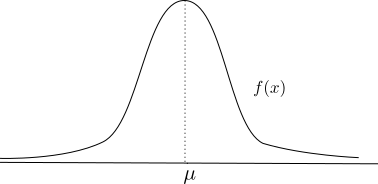
\includegraphics{normal.png}
\caption{image}
\end{figure}

Recordemos que la integral:

\[\label{int-normal}
    \int^b_a f(x) dx = \int^b_a \frac{1}{\sigma \sqrt{2\pi}} e^{-\frac{(x-\mu)^2}{2\sigma^2}} dx\]

No es más que el área bajo la curva:

\begin{figure}
\centering
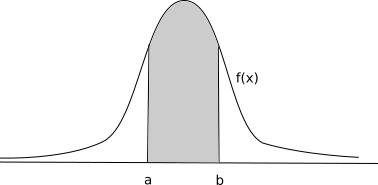
\includegraphics{drawing_ab.png}
\caption{image}
\end{figure}

Usando la formula de la normal \(N(0,1)\) dada en
(\protect\hyperlink{fz_normal}{{[}fz\_normal{]}}), definimos:
\[\Phi(y) = \int^{\infty}_{y} f(z)dz\] Que coincidirá con el área bajo
la curva:

\begin{figure}
\centering
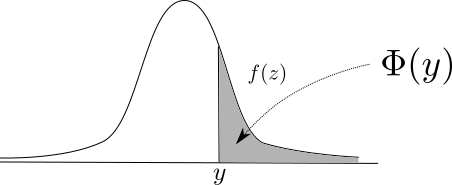
\includegraphics{drawing_phi.png}
\caption{image}
\end{figure}

Usando las propiedades de la integral definida sobre la ecuación
(\protect\hyperlink{int-normal}{{[}int-normal{]}}), se puede deducir,
haciendo el cambio de variable \(z=(x-\mu)/\sigma\) y considerando
\(z_a=(a-\mu)/\sigma\), \(z_b=(b-\mu)/\sigma\)

\[\begin{aligned}
    \label{int-normal2}
    \int^b_a f(x) dx &= \int^b_a \frac{1}{\sigma \sqrt{2\pi}} e^{-\frac{(x-\mu)^2}{2\sigma^2}} dx
    = \int^{b}_{a} \frac{1}{\sigma \sqrt{2\pi}} e^{-\frac{1}{2}\big(\frac{x-\mu}{\sigma}\big)^2} dx
    = \int^{z_b}_{z_a} \frac{1}{\sigma \sqrt{2\pi}} e^{-\frac{z^2}{2}} dz\\ 
    &= \int^{z_b}_{z_a} f(z) dz = \bigg(\int^{\infty}_{z_a} f(z) dz\bigg) - \bigg(\int^{\infty}_{z_b} f(z) dz\bigg)  = \Phi(z_a) - \Phi(z_b)\end{aligned}\]

La siguiente afirmación nos será de utilidad:

\protect\hypertarget{idea-phi-normal}{}{{[}idea-phi-normal{]}} Si una
muestra \(x_1, x_2, x_3, x_4, \ldots, x_N = (x_i)\) de \(N\) datos tiene
una distribución normal \(N(\mu, \sigma)\), entonces considerando
\(z_a=(a-\mu)/\sigma\), \(z_b=(b-\mu)/\sigma\)

\begin{enumerate}
\def\labelenumi{\arabic{enumi}.}
\item
  el numero de datos de la muestra entre a y b es
  \(N \cdot (\Phi(z_a) - \Phi(z_b))\)
\item
  el numero de datos de la muestra mayores que b es
  \(N \cdot \Phi(z_b)\)
\item
  el numero de datos de la muestra menores que b es
  \(N \cdot (1 - \Phi(z_b))\)
\end{enumerate}

Para demostrar
(\protect\hyperlink{idea-phi-normal}{{[}idea-phi-normal{]}}), basta
saber que el numero de datos de la muestra comprendidos entre dos
valores \(a\) y \(b\) es justamente el área bajo la curva normal entre
esos dos valores multiplicada por \(N\). Una vez sabido eso, basta
aplicar (\protect\hyperlink{int-normal2}{{[}int-normal2{]}}) para
deducirlo.

El hecho de que el número de valores de la muestra se relacione con el
área de la distribución normal que satisface, se puede entender si
pensamos en su histograma. En un histograma el numero de datos en un
intervalo es justamente el área del rectángulo sobre ese intervalo.

\hypertarget{cuxf3mo-calcular-usando-la-normal}{%
\section{Cómo calcular usando la
normal}\label{cuxf3mo-calcular-usando-la-normal}}

En el primer ejemplo que veremos partiremos de una distribución normal
con ciertos parámetros \(\mu\) y \(\sigma\) y nos preguntaremos cuantos
valores de la muestra están entre ciertos valores dados. En todos los
casos aplicaremos la idea
(\protect\hyperlink{idea-phi-normal}{{[}idea-phi-normal{]}})\\

La distribución de estaturas de un conjunto de 2000 personas se ajusta a
un modelo normal \(N(169cm,8cm)\). Se pide:

\begin{enumerate}
\def\labelenumi{\arabic{enumi}.}
\item
  Número de personas con una estatura superior a 191 cm.
\item
  Número de personas con una estatura inferior a 177 cm.
\item
  Número de personas con una estatura inferior a 153 cm.
\item
  Número de personas con una estatura superior a 151 cm.
\item
  Número de personas con estatura comprendida entre 171 y 175 cm.
\item
  Número de personas con estatura comprendida entre 165 y 175 cm.
\item
  Número de personas con estatura comprendida entre 157 y 167 cm.
\end{enumerate}

{a}

\begin{enumerate}
\def\labelenumi{\arabic{enumi}.}
\item
  En este caso tenemos que \(b = 191\) y \(z_b = (191-169)/8=2.75\) De
  acuerdo con lo que hemos visto en
  (\protect\hyperlink{idea-phi-normal}{{[}idea-phi-normal{]}}), basta
  con calcular \(N\cdot \Phi(z_b)= 2000\cdot \Phi(2.75)\) para obtener
  el resultado, luego hay que buscar el valor \(\Phi(2.75)\) en la
  tabla.

  Si vamos a la última página encontramos como obtener este dato. Tengo
  que buscar la fila de los dos dígitos (\(2.7\)) y luego mirar la
  columna del resto de dígitos (\(0.05\)), en este caso nos da
  \(0.00298\). Luego el numero de personas con estatura superior a 191
  es \(2000\cdot \Phi(2.75)= 2000 \cdot 0.00298= 5.95 \cong 6\)
\item
  En este caso tenemos que \(b = 177\) y \(z_b = (177-169)/8=1\) De
  acuerdo con lo que hemos visto en
  (\protect\hyperlink{idea-phi-normal}{{[}idea-phi-normal{]}}), basta
  con calcular \(N\cdot (1 - \Phi(z_b))= 2000\cdot (1-\Phi(1))\) para
  obtener el resultado, luego hay que buscar el valor \(\Phi(1)\) en la
  tabla.

  Si vamos a la última página encontramos como obtener este dato, en
  este caso nos da \(0.15866\). Luego el numero de personas con estatura
  inferior a 191 es
  \(2000\cdot (1-\Phi(1))= 2000 \cdot (1-0.15866)= 1682.7 \cong 1683\)
\item
  En este caso tenemos que \(b = 153\) y \(z_b = (153-169)/8=-2\) De
  acuerdo con lo que hemos visto en
  (\protect\hyperlink{idea-phi-normal}{{[}idea-phi-normal{]}}), basta
  con calcular \(N\cdot (1 - \Phi(z_b))= 2000\cdot (1-\Phi(-2))\) para
  obtener el resultado, luego hay que buscar el valor \(\Phi(-2)\) en la
  tabla.

  En este caso, como \(-2\) es negativo y en la tabla solo tenemos
  valores positivos, hay que saber que
  \(\phi(-2) = 1 - \Phi(2) = 1- 0.02275 = 0.099772\). Luego el numero de
  personas con estatura inferior a 153 es
  \(2000\cdot (1-\Phi(-2))= 2000 \cdot (1-0.099772)= 45.6 \cong 46\)
\item
  En este caso tenemos que \(b = 151\) y \(z_b = (151-169)/8=-2.25\) De
  acuerdo con
  (\protect\hyperlink{idea-phi-normal}{{[}idea-phi-normal{]}}), basta
  con calcular \(N\cdot \Phi(z_b)= 2000\cdot \Phi(-2.25)\) para obtener
  el resultado, luego hay que buscar el valor \(\Phi(-2)\) en la tabla.

  Al igual que antes, como \(-2\) es negativo y en la tabla solo tenemos
  valores positivos, hay que saber que
  \(\phi(-2.25) = 1 - \Phi(2.25) = 1- 0.01222 = 0.98778\). Luego el
  numero de personas con estatura superior a 153 es
  \(2000\cdot \Phi(-2.25)= 2000 \cdot 0.98778= 1975.6 \cong 1976\)
\item
  En este caso tenemos que \(b = 175, a =171\) y
  \(z_b = (175-169)/8=0.75, z_a = (171-169)/8=0.25\) De acuerdo con
  (\protect\hyperlink{idea-phi-normal}{{[}idea-phi-normal{]}}), basta
  con calcular
  \(N\cdot (\Phi(z_a) - \Phi(z_b))= 2000\cdot (\Phi(0.25) - \Phi(0.75))\)
  para obtener el resultado,

  Buscando los valores en la tabla obtenemos que el número de personas
  con estatura comprendida entre 171 y 175 es
  \(2000\cdot (\Phi(0.25) - \Phi(0.75)) = 2000 \cdot (0.40129 - 0.22965) = 343.28 \cong 343\)
\item
  En este caso tenemos que \(b = 175, a =165\) y
  \(z_b = (175-169)/8=0.75, z_a = (165-169)/8=-0.5\) De acuerdo con
  (\protect\hyperlink{idea-phi-normal}{{[}idea-phi-normal{]}}), basta
  con calcular
  \(N\cdot (\Phi(z_a) - \Phi(z_b))= 2000\cdot (\Phi(-0.5) - \Phi(0.75))\)
  para obtener el resultado, Debemos tener en cuenta que
  \(\Phi(-0.5) = 1-\Phi(0.5)= 1-0.30854 = 0.69146\) a la hora de
  buscarlo en la tabla.

  Buscando los valores en la tabla obtenemos que el número de personas
  con estatura comprendida entre 171 y 175 es
  \(2000\cdot (\Phi(-0.5) - \Phi(0.75)) = 2000 \cdot (0.69146 - 0.22965) = 923.62 \cong 924\)
\item
  En este caso tenemos que \(b = 167, a =157\) y
  \(z_b = (167-169)/8=-0.25, z_a = (157-169)/8=-1.5\) De acuerdo con
  (\protect\hyperlink{idea-phi-normal}{{[}idea-phi-normal{]}}), basta
  con calcular
  \(N\cdot (\Phi(z_a) - \Phi(z_b))= 2000\cdot (\Phi(-1.5) - \Phi(-0.25))\)
  para obtener el resultado, Debemos tener en cuenta que
  \(\Phi(-1.5) = 1-\Phi(1.5)\) y que \(\Phi(-0.25) = 1-\Phi(0.25)\) a la
  hora de buscarlo en la tabla.

  Buscando los valores en la tabla obtenemos que el número de personas
  con estatura comprendida entre 171 y 175 es
  \(2000\cdot (\Phi(-1.5) - \Phi(-0.25)) = 2000 \cdot (0.33448) = 668.96 \cong 669\)
\end{enumerate}

La distribución de pesos de un conjunto de 1000 personas se ajusta a un
modelo normal \(N(70kg,12kg)\). Se pide:

\begin{enumerate}
\def\labelenumi{\arabic{enumi}.}
\item
  Número de personas con un peso superior a 75.
\item
  Número de personas con un peso inferior a 72.
\item
  Número de personas con un peso inferior a 60.
\item
  Número de personas con un peso superior a 65.
\item
  Número de personas con un peso comprendido entre 76 y 80.
\item
  Número de personas con un peso comprendido entre 66 y 72.
\item
  Número de personas con un peso comprendido entre 50 y 60.
\end{enumerate}

La distribución de edades de un conjunto de 3000 personas se ajusta a un
modelo normal \(N(60,11)\). Se pide:

\begin{enumerate}
\def\labelenumi{\arabic{enumi}.}
\item
  Número de personas con edad superior a 65.
\item
  Número de personas con edad inferior a 62.
\item
  Número de personas con edad inferior a 50.
\item
  Número de personas con edad superior a 55.
\item
  Número de personas con edad comprendida entre 66 y 70.
\item
  Número de personas con edad comprendida entre 56 y 62.
\item
  Número de personas con edad comprendida entre 40 y 50.
\end{enumerate}

\textbf{Tabla de valores Normal \(N(0,1)\)}\\
el valor de la tabla es \(\Phi(y) = \int^{\infty}_{y} f(z)dz\). Sobre el
lado de las filas los primeros dos decimales, sobre las columnas los
siguientes.

Si queremos buscar el valor \(\Phi(0.12)\) debemos fijarnos en el valor
que está sobre la fila 2 (que comienza con \(0.1\)) y la columna 3 (que
comienza con \(+0.02\)), lo que nos da \(0.45224\)

Para valores negativos tener en cuenta que \(\Phi(-y) = 1-\Phi(y)\).
Luego si por ejemplo queremos calcular \(\Phi(-0.12)\) basta con buscar
\(\Phi(0.12)\) y luego calcular \(1-\Phi(0.12)\)\\

\begin{longtable}[]{@{}ccccccccccc@{}}
\toprule
y & +0.00 & +0.01 & +0.02 & +0.03 & +0.04 & +0.05 & +0.06 & +0.07 &
+0.08 & +0.09\tabularnewline
\midrule
\endhead
0.0 & 0.50000 & 0.49601 & 0.49202 & 0.48803 & 0.48405 & 0.48006 &
0.47608 & 0.47210 & 0.46812 & 0.46414\tabularnewline
0.1 & 0.46017 & 0.45620 & 0.45224 & 0.44828 & 0.44433 & 0.44038 &
0.43640 & 0.43251 & 0.42858 & 0.42465\tabularnewline
0.2 & 0.42074 & 0.41683 & 0.41294 & 0.40905 & 0.40517 & 0.40129 &
0.39743 & 0.39358 & 0.38974 & 0.38591\tabularnewline
0.3 & 0.38209 & 0.37828 & 0.37448 & 0.37070 & 0.36693 & 0.36317 &
0.35942 & 0.35569 & 0.35197 & 0.34827\tabularnewline
0.4 & 0.34458 & 0.34090 & 0.33724 & 0.33360 & 0.32997 & 0.32636 &
0.32276 & 0.31918 & 0.31561 & 0.31207\tabularnewline
0.5 & 0.30854 & 0.30503 & 0.30153 & 0.29806 & 0.29460 & 0.29116 &
0.28774 & 0.28434 & 0.28096 & 0.27760\tabularnewline
0.6 & 0.27425 & 0.27093 & 0.26763 & 0.26435 & 0.26109 & 0.25785 &
0.25463 & 0.25143 & 0.24825 & 0.24510\tabularnewline
0.7 & 0.24196 & 0.23885 & 0.23576 & 0.23270 & 0.22965 & 0.22663 &
0.22363 & 0.22065 & 0.21770 & 0.21476\tabularnewline
0.8 & 0.21186 & 0.20897 & 0.20611 & 0.20327 & 0.20045 & 0.19766 &
0.19489 & 0.19215 & 0.18943 & 0.18673\tabularnewline
0.9 & 0.18406 & 0.18141 & 0.17879 & 0.17619 & 0.17361 & 0.17106 &
0.16853 & 0.16602 & 0.16354 & 0.16109\tabularnewline
1.0 & 0.15866 & 0.15625 & 0.15386 & 0.15151 & 0.14917 & 0.14686 &
0.14457 & 0.14231 & 0.14007 & 0.13786\tabularnewline
1.1 & 0.13567 & 0.13350 & 0.13136 & 0.12924 & 0.12714 & 0.12507 &
0.12302 & 0.12100 & 0.11900 & 0.11702\tabularnewline
1.2 & 0.11507 & 0.11314 & 0.11123 & 0.10935 & 0.10749 & 0.10565 &
0.10383 & 0.10204 & 0.10027 & 0.09853\tabularnewline
1.3 & 0.09680 & 0.09510 & 0.09342 & 0.09176 & 0.09012 & 0.08851 &
0.08692 & 0.08534 & 0.08379 & 0.08226\tabularnewline
1.4 & 0.08076 & 0.07927 & 0.07780 & 0.07636 & 0.07493 & 0.07353 &
0.07215 & 0.07078 & 0.06944 & 0.06811\tabularnewline
1.5 & 0.06681 & 0.06552 & 0.06426 & 0.06301 & 0.06178 & 0.06057 &
0.05938 & 0.05821 & 0.05705 & 0.05592\tabularnewline
1.6 & 0.05480 & 0.05370 & 0.05262 & 0.05155 & 0.05050 & 0.04947 &
0.04846 & 0.04746 & 0.04648 & 0.04551\tabularnewline
1.7 & 0.04457 & 0.04363 & 0.04272 & 0.04182 & 0.04093 & 0.04006 &
0.03920 & 0.03836 & 0.03754 & 0.03673\tabularnewline
1.8 & 0.03593 & 0.03515 & 0.03438 & 0.03362 & 0.03288 & 0.03216 &
0.03144 & 0.03074 & 0.03005 & 0.02938\tabularnewline
1.9 & 0.02872 & 0.02807 & 0.02743 & 0.02680 & 0.02619 & 0.02559 &
0.02500 & 0.02442 & 0.02385 & 0.02330\tabularnewline
2.0 & 0.02275 & 0.02222 & 0.02169 & 0.02118 & 0.02068 & 0.02018 &
0.01970 & 0.01923 & 0.01876 & 0.01831\tabularnewline
2.1 & 0.01786 & 0.01743 & 0.01700 & 0.01659 & 0.01618 & 0.01578 &
0.01539 & 0.01500 & 0.01463 & 0.01426\tabularnewline
2.2 & 0.01390 & 0.01355 & 0.01321 & 0.01287 & 0.01255 & 0.01222 &
0.01191 & 0.01160 & 0.01130 & 0.01101\tabularnewline
2.3 & 0.01072 & 0.01044 & 0.01017 & 0.00990 & 0.00964 & 0.00939 &
0.00914 & 0.00889 & 0.00866 & 0.00842\tabularnewline
2.4 & 0.00820 & 0.00798 & 0.00776 & 0.00755 & 0.00734 & 0.00714 &
0.00695 & 0.00676 & 0.00657 & 0.00639\tabularnewline
2.5 & 0.00621 & 0.00604 & 0.00587 & 0.00570 & 0.00554 & 0.00539 &
0.00523 & 0.00508 & 0.00494 & 0.00480\tabularnewline
2.6 & 0.00466 & 0.00453 & 0.00440 & 0.00427 & 0.00415 & 0.00402 &
0.00391 & 0.00379 & 0.00368 & 0.00357\tabularnewline
2.7 & 0.00347 & 0.00336 & 0.00326 & 0.00317 & 0.00307 & 0.00298 &
0.00289 & 0.00280 & 0.00272 & 0.00264\tabularnewline
2.8 & 0.00256 & 0.00248 & 0.00240 & 0.00233 & 0.00226 & 0.00219 &
0.00212 & 0.00205 & 0.00199 & 0.00193\tabularnewline
2.9 & 0.00187 & 0.00181 & 0.00175 & 0.00169 & 0.00164 & 0.00159 &
0.00154 & 0.00149 & 0.00144 & 0.00139\tabularnewline
3.0 & 0.00135 & 0.00131 & 0.00126 & 0.00122 & 0.00118 & 0.00114 &
0.00111 & 0.00107 & 0.00104 & 0.00100\tabularnewline
3.1 & 0.00097 & 0.00094 & 0.00090 & 0.00087 & 0.00084 & 0.00082 &
0.00079 & 0.00076 & 0.00074 & 0.00071\tabularnewline
3.2 & 0.00069 & 0.00066 & 0.00064 & 0.00062 & 0.00060 & 0.00058 &
0.00056 & 0.00054 & 0.00052 & 0.00050\tabularnewline
3.3 & 0.00048 & 0.00047 & 0.00045 & 0.00043 & 0.00042 & 0.00040 &
0.00039 & 0.00038 & 0.00036 & 0.00035\tabularnewline
3.4 & 0.00034 & 0.00032 & 0.00031 & 0.00030 & 0.00029 & 0.00028 &
0.00027 & 0.00026 & 0.00025 & 0.00024\tabularnewline
3.5 & 0.00023 & 0.00022 & 0.00022 & 0.00021 & 0.00020 & 0.00019 &
0.00019 & 0.00018 & 0.00017 & 0.00017\tabularnewline
3.6 & 0.00016 & 0.00015 & 0.00015 & 0.00014 & 0.00014 & 0.00013 &
0.00013 & 0.00012 & 0.00012 & 0.00011\tabularnewline
3.7 & 0.00011 & 0.00010 & 0.00010 & 0.00010 & 0.00009 & 0.00009 &
0.00008 & 0.00008 & 0.00008 & 0.00008\tabularnewline
3.8 & 0.00007 & 0.00007 & 0.00007 & 0.00006 & 0.00006 & 0.00006 &
0.00006 & 0.00005 & 0.00005 & 0.00005\tabularnewline
3.9 & 0.00005 & 0.00005 & 0.00004 & 0.00004 & 0.00004 & 0.00004 &
0.00004 & 0.00004 & 0.00003 & 0.00003\tabularnewline
4.0 & 0.00003 & 0.00003 & 0.00003 & 0.00003 & 0.00003 & 0.00003 &
0.00002 & 0.00002 & 0.00002 & 0.00002\tabularnewline
\bottomrule
\end{longtable}
